\documentclass[10pt, letterpaper]{article}
\usepackage[top=80pt,bottom=80pt,left=60pt,right=60pt]{geometry}
\usepackage{tabularx}
\usepackage{float}
\usepackage{amsmath} % for boxing equations
\usepackage{titling}
\newcommand{\subtitle}[1]{
  \posttitle{
    \par\end{center}
    \begin{center}\large#1\end{center}
    \vskip0.5em}
}
\usepackage{tikz}
\usepackage[section]{placeins}
\usepackage[utf8]{inputenc}
\usepackage{pgfplots} % for table
\usepackage{pgfplotstable} % for linear regression
\usepackage{csvsimple}
\usepackage{subfig}
\usepackage{setspace} % line spacing
\doublespacing

\begin{document}

  \title{The Monte Carlo Method}
  \subtitle {IB Math HL Period 5, Dr. Silverman}
  \date{16 November 2015}
  \author{Jackson Chen}
  \maketitle

  \section{Introduction}

  \subsection{Personal Engagement}

  I have always learned to solve numeric problems, such as calculating the area of a shape in Euclidean geometry,
  with a deterministic formulaic method. This may consist of using numeric relationships or calculus. However, I became fascinated with
  the Monte Carlo method after learning about it from a professor. I had never thought of applying probability to numeric problems
  with seemingly definite solutions until then. The Monte Carlo method will be described in more detail in Section \ref{subsec:explanation}.
  This method is also surprisingly straightforward compared to some of
  the other methods used to solve numeric problems, and may have even an advantage when finding areas of irregular shapes.

  \subsection{Explanation} \label{subsec:explanation}

  The Monte Carlo method consists of using random sampling in order to solve numerical problems. This may seem like an imprecise method
  of solving, for example, the area of a circle. However, there are two crucial criteria to consider when using the Monte Carlo method:
  \begin{itemize}
    \item The greater the number of random inputs that are chosen, the greater the accuracy
    \item The more uniform the distribution of random samples, the more accurate the final answer
  \end{itemize}

  In order to address the second point made in the list above, one may assume that truly random numbers are needed to ensure a fair distribution.
  However, this is not the case as pseudorandom number generation, which is prevalent in many number generator algorithms, should be satisfactory
  for the usage of the Monte Carlo method.

  \section{History}

  Before the Monte Carlo method, statistical sampling was used to estimate uncertainties in simulations. The Monte Carlo method
  reversed this approach, using probabilistic analogs to solve deterministic problems.

  The earliest variant of the Monte Carlo method can be seen in the Buffon's needle experiment in the 18th century where $\pi$ was estimated
  by dropping needles on a floor made of equidistant and parallel strips.\footnote{"The Beginning of the Monte Carlo Method" by N. Metropolis, 1987}

  However, the current version of the Monte Carlo method was created in the late 1940's by Stanislaw Ulam while working on
  a nuclear weapons project. He was trying to investigate radiation shielding and the distance neutrons would likely travel through various
  materials. Despite his team obtaining all of the necessary data, the physicists were unable to solve the problem using a conventional deterministic
  method. Ulam thought of using random experiments. He generated the pseudorandom numbers using the middle-square method, the quickest at his
  disposal. Monte Carlo was the code name of the work, due to the level of secrecy required, and the name stuck.\footnote{"Stan Ulam, John von
  Neumann and the Monte Carlo Method" by Roger Eckhardt, 1987}

  The Monte Carlo methods were widely used in the Manhattan Project, and used in the development of the hydrogen bomb. The Rand Corporation
  and the US Air Force widely funded work on Monte Carlo methods during this time, broadening its applications to various other fields.

  \section{Calculation} \label{sec:usage}

  A sample calculation for the Monte Carlo Method will be performed to calculate the area of a circle. This will be done to demonstrate the properties of
  the method.

  \begin{figure}
    \centering
    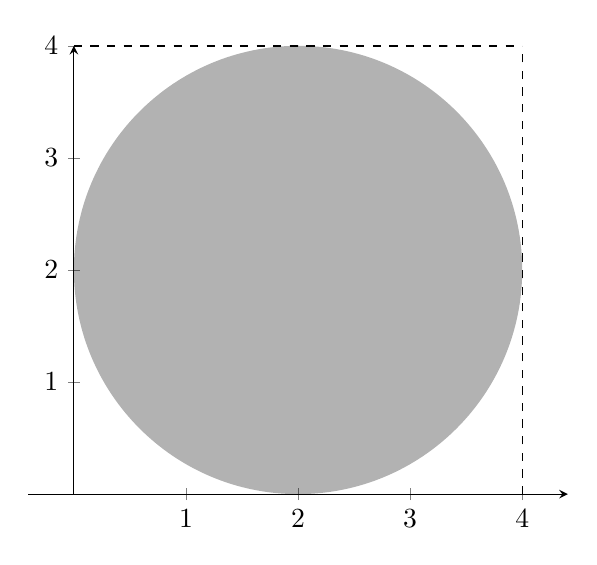
\begin{tikzpicture}
      \begin{axis}[
        xmin=0,
        xmax=4,
        ymin=0,
        ymax=4,
        axis equal,
        axis lines=middle,
        disabledatascaling]

      \fill [opacity=0.3] (2, 2) circle [radius=2];
      \addplot[thick, dashed, domain=0:4] {4};
      \addplot[dashed] coordinates{(4,0) (4,4)};
      \end{axis}
    \end{tikzpicture}
    \caption{A circle with center (2, 2) and radius 2 used in the sample calculation} \label{fig:circle}
  \end{figure}

  The circle is centered at (2, 2) and has radius 2. Thus the equation for the circle is given with
  \[ (x-2)^2 + (y-2)^2 = 4 \]
  The domain of possible inputs consists of the square bounded by the x and y axes and the lines
  $x = 4$ and $y = 4$ as represented by the dashed lines in Figure \ref{fig:circle}. \\

  Using the standard area of a circle equation, the exact value for the area can be found:

  \[ A = \pi r^2 = 4\pi \approx 12.566 \]

  Now to calculate the area using the Monte Carlo method, a computer program will be used to generate several thousand
  points within the domain.

  The program uses the \texttt{random} Python library, which implements psuedo-random number generation.
  This library generates random floats uniformly in the range $[0, 1)$. Since Python uses Mersenne Twister as the core generator,
  it produces 53-bit precision floats with a period of $2^{19937} - 1$.\footnote{https://docs.python.org/2/library/random.html}
  Despite the fact that the generator is not perfectly random, the \texttt{random} library satisfies the second criterion mentioned
  in Section \ref{subsec:explanation}.


  \begin{table}[H]
    \centering
    \begin{tabularx}{\linewidth}{>{\centering\arraybackslash}X>{\centering\arraybackslash}X>{\centering\arraybackslash}X>{\centering\arraybackslash}X>{\centering\arraybackslash}X }
      \hline \textbf{Number of test points} & \textbf{Points in circle} & \textbf{Percent of Domain} & \textbf{Predicted Area} & \textbf{Percent Error} \\ \hline
              10                            &	7                         & 70.0\%                      & 11.200                  & 10.9\%            \\ \hline
              20                            &	15                        & 75.0\%                      & 12.000                  & 4.50\%            \\ \hline
              50                            &	39                        & 78.0\%                      & 12.480                  & 0.684\%            \\ \hline
              100                           &	78                        & 78.0\%                      & 12.480                  & 0.684\%            \\ \hline
              500                           &	393                       & 78.6\%                      & 12.576                  & 0.0796\%            \\ \hline
              1000                          &	785                       & 78.5\%                      & 12.560                  & 0.0477\%            \\ \hline
              2000                          & 1570                      & 78.5\%                      & 12.560                  & 0.0477\%            \\ \hline
              5000                          & 3927                      & 78.5\%                      & 12.560                  & 0.0477\%            \\ \hline
              10000                         & 7850                      & 78.5\%                      & 12.560                  & 0.0477\%            \\ \hline
              50000                         & 39272                     & 78.5\%                      & 12.560                  & 0.0477\%            \\ \hline
              100000                        & 78539                     & 78.5\%                      & 12.560                  & 0.0477\%            \\ \hline
    \end{tabularx}
    \caption{Predicted area and its accuracy for a varying number of test points.}
    \label{tab:data}
  \end{table}

  It took a computer approximately 101.5 seconds to generate 100000 points. Thus, the maximum test points generated was
  capped at 100000 for the sake of time and because additional points were yielding negligible changes in predicted area accuracy.

  The predicted area is calculated by taking the percent of the domain (which is the percent of the total random samples that are in the circle)
  and multiplying it by the area of the domain, in this case, a square with area 16.

  The data in \ref{tab:data} reflects the first criterion in Section \ref{subsec:explanation}. The greater the number of test points,
  the smaller the percent error and thus the more accurate the predicted area is. Once enough points were used, the percent error became
  less than half of a percent.

  In the previous situation, it seemed disadvantageous to use the Monte Carlo method in order to calculate the area of the sphere. It requires
  more computing time and power than using the deterministic numerical calculation. This may be true for simple cases such as that. However,
  in the cases of integration with hundreds of degrees of freedom (or dimensions), the curse of dimensionality\footnote{Richard Ernest Bellman;
  Rand Corporation (1957). Dynamic programming. Princeton University Press.} dictates an exponential increase in complexity as the number of
  dimensions rises when using deterministic numerical integration. Using the Monte Carlo method instead would prevent the exponential increase
  in computational time. According to the central limit theorem, quadrupling the number of samples would halve the error irrespective of the
  number of dimensions.

  \section{Applications}

  The Monte Carlo method has a wide array of applications in science, engineering, and computing. For example, it is used in ensemble models to
  help with weather forecasting. In this case, multiple predictions are made with slightly different initial conditions that may result from
  past observations. The multifarious simulations are used to account for errors that would be introduced through the use of imperfect conditions
  and imperfections in the model formulation. In addition, this type of simulation is also sometimes used during wartime in order to calculate
  the position of enemy aircraft in the skies.

  Computer graphics use Monte Carlo Ray Tracing to render three dimensional scenes by randomly tracing samples of paths of light. This can be
  used in applications like first person video games, where Monte Carlo simulations help determine if the enemies or objects behind walls
  can be seen from the perspective of the player through path tracing. Simulations with a massive amount of samples on pixels allow the sample
  average to converge to the solution of the rendering solution, thus making Monto Carlo simulations one of the most accurate three
  dimensional graphics rendering methods.

  In addition to rendering games, Monte Carlo Tree Search (MCTS) has allowed for bots for games to search for the best move in
  any given situation. MCTS has been successfully used in Go, Tantrix, and Battleship.

  \section{Conclusion}

  The Monte Carlo method provides an alternative to the conventional deterministic numerical computations used to solve a vast array of
  math problems, including area calculation and integration. In situations where the complexity of the problem exponentially grows when
  using deterministic methods, such as using numerical integration for functions in many dimensions, the Monte Carlo method typically
  becomes advantageous.

  The Monte Carlo method has a plethora of applications that revolutionized various fields in science, as well as human wartime tactics.
  It provides the most accurate way of rending three dimensional graphics, revolutionized path finding algorithms for computer bots, and
  allows for the prediction of weather that accounts for the uncertainty unsolved for in conventional methods.

  Through investigating Monte Carlo simulations, I have grown as a mathematician, in terms of broadening my ability to solve deterministic
  problems in an unconventional manner. With my new knowledge, I can fully appreciate the widespread applications that math entails in my daily
  life. The multidisciplinary approach taken with this method has driven me to continue researching this topic, as I have experience
  in many fields of that have been influenced by this method.

\end{document}
